\documentclass[parskip=full, a4paper]{scrreprt}

%%% PACKAGES %%%

% add unicode support and use german as language
\usepackage[utf8]{inputenc}
\usepackage[ngerman]{babel}

% Use Helvetica as font
\usepackage[scaled]{helvet}
\renewcommand\familydefault{\sfdefault}
\usepackage[T1]{fontenc}

% Better tables
\usepackage{tabularx}

% Better enumerisation env
\usepackage{enumitem}

% Use graphics
\usepackage{graphicx}

% Have subfigures and captions
\usepackage{subcaption}

% Be able to include PDFs in the file
\usepackage{pdfpages}

% Have custom abstract heading
\usepackage{abstract}

% Need a list of equation
\usepackage{tocloft}
\usepackage{ragged2e}

% Better equation environment
\usepackage{amsmath}

% Symbols for most SI units
\usepackage{siunitx}

\usepackage{csquotes}

% Clickable Links to Websites and chapters
\usepackage{hyperref}

% Change page rotation
\usepackage{pdflscape}

% Symbols like checkmark
\usepackage{amssymb}
\usepackage{pifont}

\usepackage[absolute]{textpos}

% Glossary, hyperref, babel, polyglossia, inputenc, fontenc must be loaded before this package if they are used
\usepackage{glossaries}
% Redefine the quote charachter as we are using ngerman
\GlsSetQuote{+}
% Define the usage of an acronym, Abbreviation (Abbr.), next usage: The Abbr. of ...
\setacronymstyle{long-short}

% Bibliography & citing
\usepackage[
backend=biber,
style=apa,
bibstyle=apa,
citestyle=apa,
sortlocale=de_DE
]{biblatex}
\addbibresource{Referenzen.bib}
\DeclareLanguageMapping{ngerman}{ngerman-apa}

%%% TOC Header
\addto\captionsngerman{
	\renewcommand{\contentsname}{Traktanden}
}

%%% Not clearpage before chapter
\usepackage{etoolbox}
\makeatletter
\patchcmd{\scr@startchapter}{\if@openright\cleardoublepage\else\clearpage\fi}{}{}{}
\makeatother
%%% DOCUMENT %%%

\begin{document}
\begin{titlepage}
\vspace*{2.5cm}
\noindent
\Huge{\textbf{Sitzungsprotokoll SprintReview}} \\
\noindent
\Large{19.03.2019, Rotkreuz}\\
\vfill
\noindent
\large{Author: Dane Wicki}\\
\noindent
\large{Datum: \today}\\
\end{titlepage}

\noindent
\begin{tabularx}{\textwidth}{XXl}
\hline \\
\multicolumn{3}{l}{\Large{\textbf{SprintReview  Bachelorarbeit}}}\\
\multicolumn{3}{l}{Suche von mit RFID ausgerüsteten Einzelexemplaren} \\ \\
\hline 
	Freitag, & & Hochschule Luzern \\
	19. März 2019 & 08:00 Uhr bis 09:30 Uhr & Raum 41.412 - 8, Rotkreuz \\
\hline \\
\hline
Besprechungsart & SprintReview & \\ 
\hline 
Besprechungsleiter & Pascal Baumann & \\ 
\hline 
Protokollführer & Dane Wicki & \\ 
\hline 
Teilnehmer & Mike Märki & \\ & Pascal Baumann & \\ & Dane Wicki & \\
\hline 
Abwesend & Prof. Martin Jud & \\ 
\hline 
\end{tabularx} 
	
	\noindent

\tableofcontents
\chapter{Protokoll und Aufgabenstellung}

Es wurde kurz das Protokoll der letzten auf Sitzung gegengefragt ob dieses so korrekt sei. Herr Märki bestätigte, die Korrektheit des Protokolls. 

Pascal Baumann legte Herr Märki die konkrete Aufgabenstellung zur Unterschrift bereit. Herr Märki unterzeichnete diese. 

\chapter{Präsentation der Sprint Resultate}

Herr Wicki begann mit dem Vorzeigen des Ablaufes der Sprints.  
Es wurde erklärt, dass ein Sprint 2 Wochen dauert, und all 4 Wochen ein Meeting mit Herr Märki angestrebt wird. 

\chapter{Präsentation Konzept 1}

Herr Wicki stellte das Ziel des 1. Konzeptes vor, dass ein bestimmtes, bekanntes Exemplar im Hochregallager deplatziert wurde. Er führte weiter an, dass ein solcher Fall eintreten könnte, würde ein Exemplar von der Speicherbiliothek bestellt und dieses nicht im entsprechenden Behälter vorhanden wäre. Das Exemplar muss dementsprechend im Hochregallager zu finden sein. 
Weiter sagte er, dass in diesem Konzept ein Spezieller Behälter entwickelt werden, welche ins Hochregallager gesendet werden kann. Weiter führte er an, dass nur genau ein Exemplar abgesucht werden kann, da diese Methodik Geschwindigkeitsvorteile bietet. Herr Märke fragte ob der Grund für diese Geschwindigkeitsvorteile niedergeschrieben wurden. Herr Wicki bestätigte, dass dies im Konzept beschrieben ist.  

Herr Baumann erklärte darauf noch den Suchalgorithmus von RFID HF. Er erklärte, dass bei RFID HF ein Detection Prevention Algorithmus zum Einsatz komme. Dieser würde die Tags mittels einer Maskierung anfragen. Trifft diese Maske auf einen Tag zu würde dieser Antworten. Trifft er auf mehrere zu detektiert das Lesegerät eine Kollision und definiert die Eingabemaske genauer, bis nur ein Tag dieser Maske entspricht. Weiter führte Herr Baumann auf, dass sofern die ID eines Tags bekannt sei der Algorithmus nicht gebraucht werden würde, da nur ein Tag antworten kann. Dies würde zu einem schnelleren auffinden des Tags führen. 

Herr Märki fragte nach, ob es eine Möglichkeit gäbe in den Raum zu fragen, welche Tags vorhanden seien, Herr Baumann erklärte, dass dies nicht möglich sei. 

Herr Wicki führte nochmals nach, dass nur ein Tag auf einmal gelesen werden können, ansonsten empfängt man nicht spezifizierbare Daten. 
Herr Wicki erklärte, dass das im Konzept Spezifizierte Lesemodul mit dem Gebrauch des Prävention Algorithmus 50 Tags in der Sekunde lesen könne, weshalb es für einen Tag nicht länger gehen kann als 1/50 Sekunden. 

Herr Märki fragt ob dieser Algorithmus spezifiziert sei. Herr Baumann erwiderte, dass diese in der ISO Norm genau spezifiziert sind. 
Weiter fragte Herr Märki ob nicht Mehrere Tags aufs mal gelesen werden könne, Herr Wicki erwiederte, dass der Roboter eine Geschwindigkeit von maximal 24m/s haben dürfte, wenn nur ein Tag gelesen werden würde. Der Roboter bewege sich jedoch nur 6m/s womit bei dieser geringeren Geschwindigkeit 3 Tags auf einmal abgesucht werden können. 
Herr Märki führte noch an, dass es sehr aufwändig ist in der Gasse nach einem Exemplar zu suchen, daher wäre es nützlich könne man gleich mehrere Tags absuchen. 

Herr Wicki erklärte anschliessend, dass in diesem Konzept 2 Suchmodi zum Einsatz kämen. Dies aus dem Grund, dass RFID HF eine Theoretische Maximale Distanz von 1m beträgt. Die Distanz im Hochregallager beträgt jedoch 1.2m, da zwei Behälter jeweils hintereinander gelagert werden. Es ist in diesem Konzept dementsprechend nicht möglich mit der Vorbeifahrt die Tags der hinteren Box herauszulesen. Daher kämen zwei Suchmodi zum Einsatz, der Erste würde eine Oberflächliche Suche starten, welche lediglich den vorderen Behälter nach dem Tag absucht. Somit könnte eine Abdeckung von ca. 50\% gewährleistet werden. 
Weiter führte Herr Wicki auf, dass für den ersten Suchmodus dieses Konzeptes mehrere Antennen um die Rechte wie auch die Linke Gasse simultan auslesen zu können. Die Dauer dieses Suchmodus Beträge gut drei Minuten pro Gasse. 

Herr Märki stellte anschliessend die Frage, ob der Roboter auch in der Höhe die Behälter absucht. Herr Wicki verwies auf die Graphik \ref{fig:antennenpos}, auf welcher aufgezeigt wird, dass bei Position 2 und 3 die Obere wie auch die Untere Reihe zur Selben Zeit gelesen werden sollen um so nur jede 3 Reihe durchfahren zu müssen. Dies müsse jedoch in einem Proof of Concept evaluiert werden.
Herr Märki stellte fest, dass die Positionierung der Pos. 3 Direkt auf das Metall des Roboters ausgerichtet wäre. Herr Baumann erwiederte, dass ein Vorteil von RFID HF gegenüber RFID UHF in der geringen Störung durch Metall liegt.

\begin{figure}
	\centering
	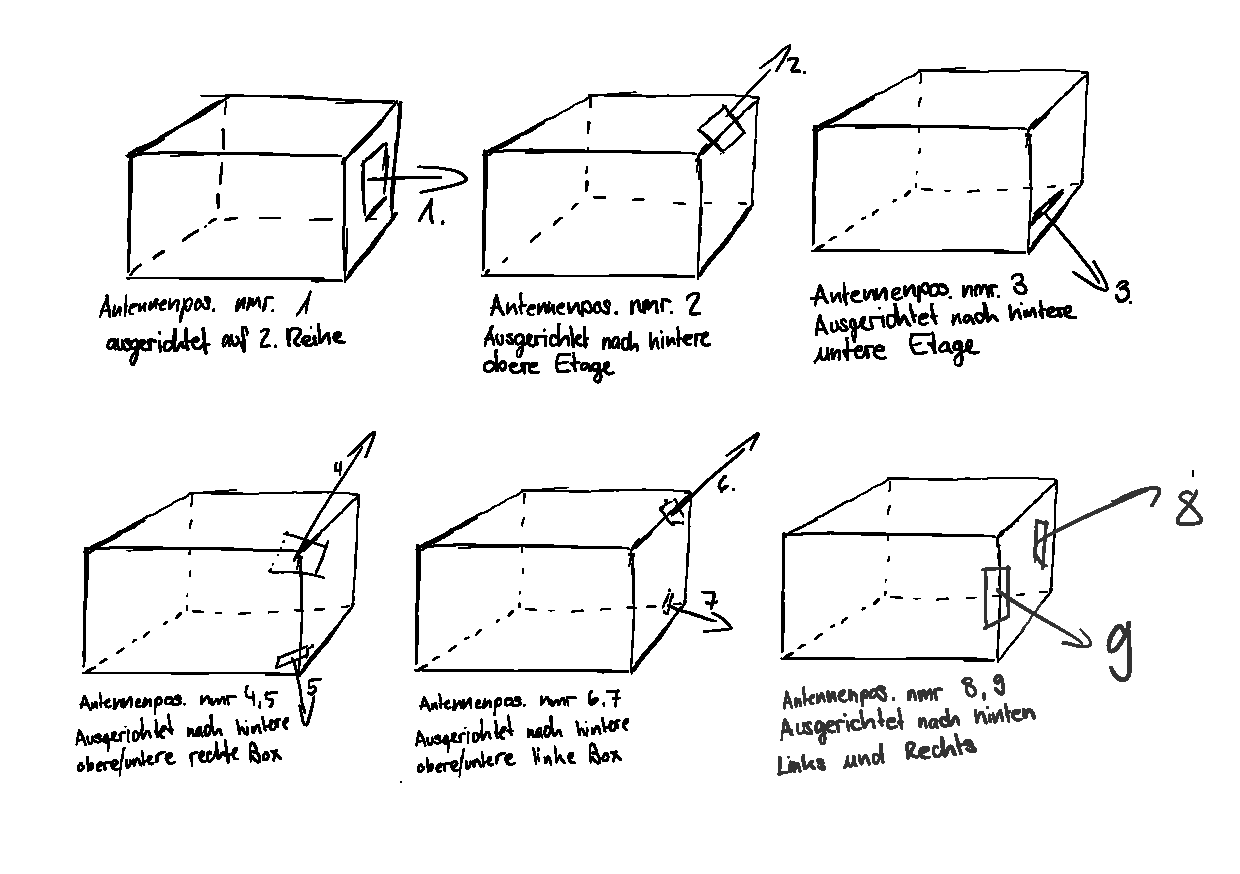
\includegraphics[keepaspectratio, width=0.8\linewidth]{images/Konzept_1_Drawings3.pdf}
	\caption{Positionen der Antennen}
	\label{fig:antennenpos}
\end{figure}

Herr Wicki erklärte weiter, dass beim Suchmodus Nummer zwei die Boxen der vorderen Reihe ausgetauscht werden würden. Dazu müsste gemäss diesen Konzeptes die bestehende Verwaltungssoftware erweitert werden. Damit der Roboter autonom die Boxen absuchen könnte. Herr Wicki führte auf, dass dieser Suchvorgang ca. 4h dauert pro Reihe, sofern der Austausch 2er Boxen nicht länger als 10s betrage. Sobald der Lesebehälter die Position eines Vorderen Behälters eingenommen hat sollen gleich alle neun hinteren Behälter ausgelesen werden gemäss den Antennenpositionen auf \ref{fig:antennenpos}. Somit kann eine Geschwindigkeitssteigerung des Faktors 9 erreicht werden. Der Vorteil dieses Konzeptes läge in der Abdeckung von bis zu 100\%. Herr Wicki fasste zusammen, dass die Störung durch Metall wie auch die Interferencen mehrere Antennen noch in einem Proof of Concept eruiert werden müssen. Und eben diese Faktoren sehr grosses Fehlerpotential in diesem Konzept aufweisen.

Herr Wicki zeigte nochmals die Antennenpositionen auf der Graphik \ref{fig:antennenpos}. Dabei sollen die Positionen 4 - 6 Lediglich für den zweiten Suchmodus verwendet werden.
Herr Märki fragte darauf, ob beide Reihen gelesen werden können. Herr Wicki bestätigte dies, dass bei Suchmodus zwei Beide Reihen gelesen werden könnten.
Herr Baumann Zweichnete anschliessend eine Graphik (wie Graphik \ref{fig:boxenposition}), welche die Position der Box veranschaulicht. Dabei erklärte er, dass die 9 Hinteren 9 Boxen simultan gelesen werden.

\begin{figure}
	\centering
	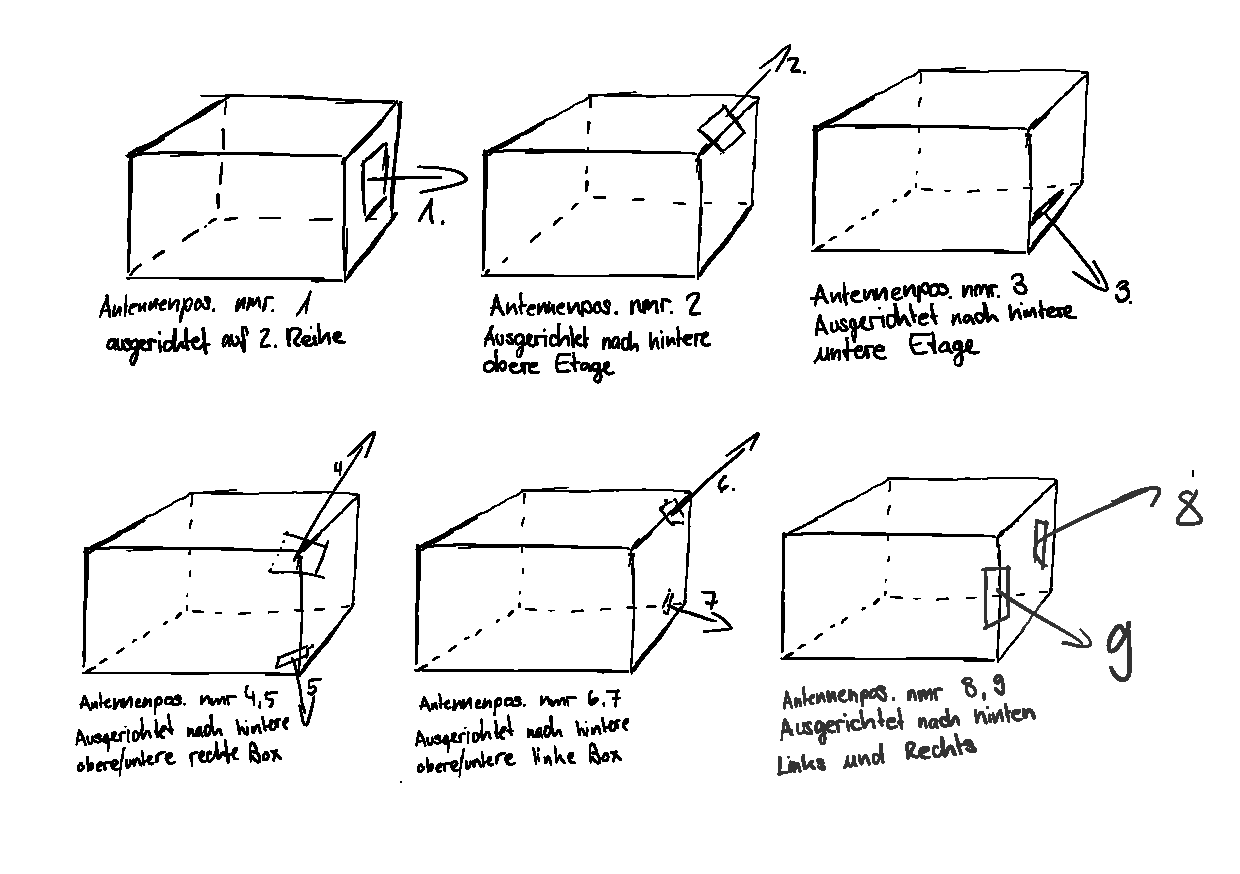
\includegraphics[keepaspectratio, width=0.8\linewidth]{images/Konzept_1_Drawings3.pdf}
	\caption{Positionen der Antennen}
	\label{fig:antennenpos}
\end{figure}

Herr Märki wies dabei noch darauf hin, dass die Positionen der Behälter nicht fix ist, sie also über den Tag an neue Positionen gelangen können. Herr Wicki erklärte, dass diese nur beim Zeitpunkt der Auslese relevant sei, da anschliessend mit der Behälter ID gearbeitet werden sollen.
Her Märki fragte anschliessen, dass man so jedoch wissen müsse, welcher Behälter sich auf einer Bestimmten Position befinden würde. Herr Wicki wie Herr Baumann bestätigten dies.




















% Herr Märki wies dabei noch darauf hin, dass es momentan keine Möglichkeit gäbe die Positionen zu kennen, da diese flüchtig seien. Herr Wicki entgegnete, dass eine Voraussetzung für dieses Konzept eine entsprechende Anpassung der Lagerverwaltungssoftware beinhalte, bei welcher es teilweise um genau jenes Problem handle.


\chapter{Präsentation Konzept 2}



\end{document}